% Compile as a standalone figure with pdflatex or tectonic.
\documentclass[tikz,border=10pt]{standalone}
\usetikzlibrary{arrows.meta,calc}

\definecolor{ink}{HTML}{18334A}
\definecolor{lineblue}{HTML}{486780}
\definecolor{paperblue}{HTML}{EDF4F9}
\definecolor{teal}{HTML}{21645C}
\definecolor{paperteal}{HTML}{EBF5F0}
\definecolor{amber}{HTML}{84581D}
\definecolor{paperamber}{HTML}{FFF5E5}

\newcommand{\heading}[1]{\mbox{\fontsize{11}{13}\selectfont\bfseries #1}}
\begin{document}
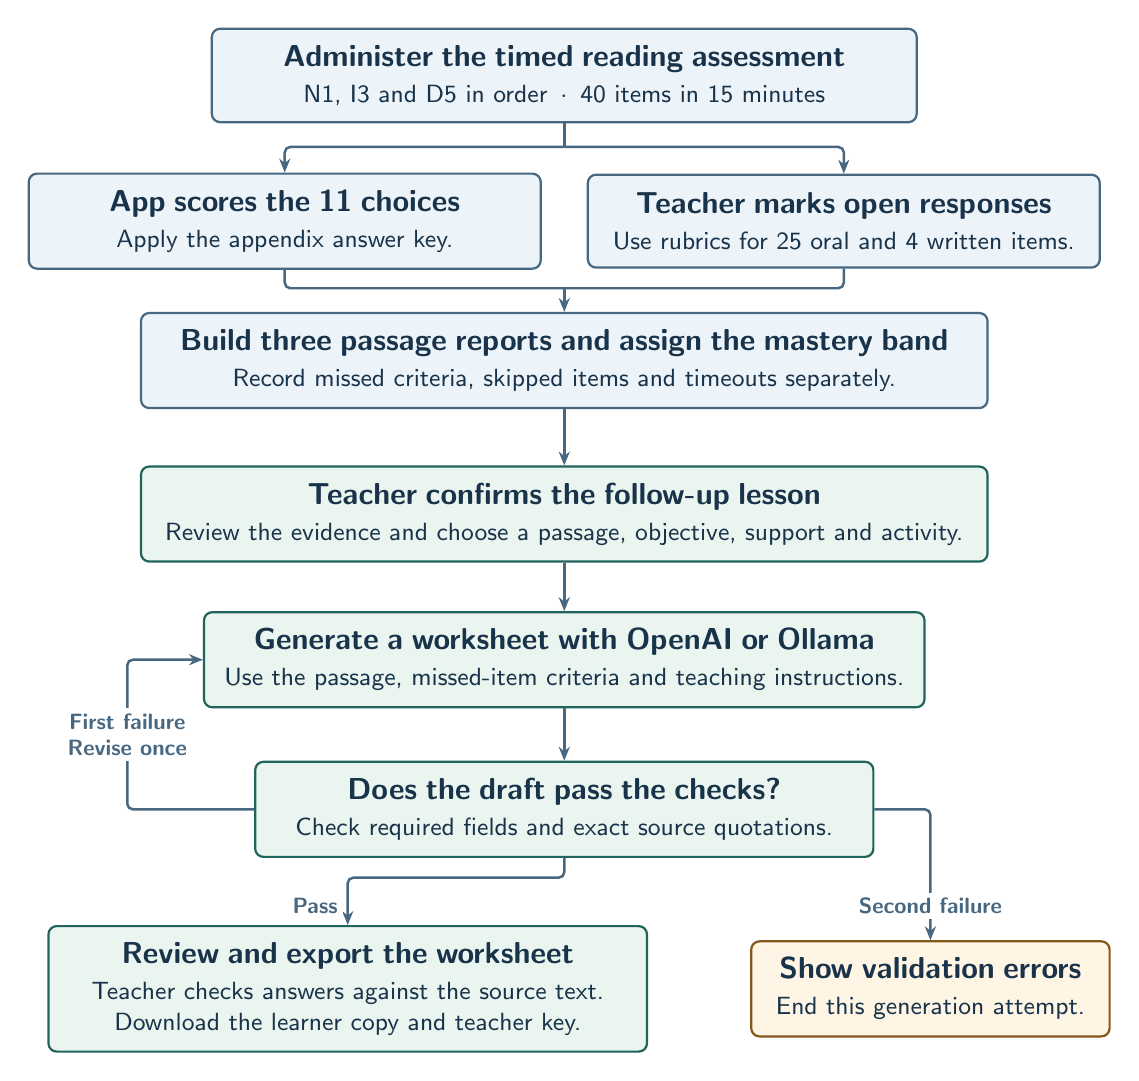
\begin{tikzpicture}[
  font=\sffamily\small, text=ink,
  card/.style={draw=lineblue, fill=paperblue, line width=.8pt,
    rounded corners=3pt, align=center, inner xsep=5pt, inner ysep=6pt},
  lesson/.style={card, draw=teal, fill=paperteal},
  issue/.style={card, draw=amber, fill=paperamber},
  flow/.style={-{Stealth[length=5pt,width=4pt]}, draw=lineblue,
    line width=.9pt, rounded corners=2pt},
  outcome/.style={font=\sffamily\footnotesize\bfseries, fill=white,
    inner sep=2pt, text=lineblue}
]
  \node[card, text width=8.6cm] (form) at (0,0)
    {\heading{Administer the timed reading assessment}\\[2pt]
     N1, I3 and D5 in order\enspace$\cdot$\enspace40 items in 15 minutes};

  \node[card, text width=6.15cm, minimum height=1.18cm] (choice) at (-3.55,-1.85)
    {\heading{App scores the 11 choices}\\[2pt]
     \mbox{Apply the appendix answer key.}};
  \node[card, text width=6.15cm, minimum height=1.18cm] (rubric) at (3.55,-1.85)
    {\heading{Teacher marks open responses}\\[2pt]
     \mbox{Use rubrics for 25 oral and 4 written items.}};
  \coordinate (split) at ($(form.south)+(0,-.30)$);
  \draw[draw=lineblue,line width=.9pt] (form.south) -- (split);
  \draw[flow] (split) -| (choice.north);
  \draw[flow] (split) -| (rubric.north);

  \node[card, text width=10.4cm] (report) at (0,-3.62)
    {\heading{Build three passage reports and assign the mastery band}\\[2pt]
     \mbox{Record missed criteria, skipped items and timeouts separately.}};
  \coordinate (join) at ($(report.north)+(0,.30)$);
  \draw[draw=lineblue,line width=.9pt,rounded corners=2pt]
    (choice.south) |- (join) -| (rubric.south);
  \draw[flow] (join) -- (report.north);

  \node[lesson, text width=10.4cm] (plan) at (0,-5.57)
    {\heading{Teacher confirms the follow-up lesson}\\[2pt]
     \mbox{Review the evidence and choose a passage, objective, support and activity.}};
  \draw[flow] (report) -- (plan);

  \node[lesson, text width=8.8cm] (draft) at (0,-7.42)
    {\heading{Generate a worksheet with OpenAI or Ollama}\\[2pt]
     \mbox{Use the passage, missed-item criteria and teaching instructions.}};
  \draw[flow] (plan) -- (draft);

  \node[lesson, text width=7.5cm] (check) at (0,-9.32)
    {\heading{Does the draft pass the checks?}\\[2pt]
     Check required fields and exact source quotations.};
  \draw[flow] (draft) -- (check);
  \coordinate (retry) at (-5.55,-9.32);
  \draw[flow] (check.west) -- (retry) |- (draft.west);
  \node[outcome,align=center] at (-5.55,-8.37)
    {First failure\\Revise once};

  \node[lesson, text width=7.25cm] (export) at (-2.75,-11.60)
    {\heading{Review and export the worksheet}\\[2pt]
     \mbox{Teacher checks answers against the source text.}\\
     \mbox{Download the learner copy and teacher key.}};
  \node[issue, text width=4.2cm] (stop) at (4.65,-11.60)
    {\heading{Show validation errors}\\[2pt]
     End this generation attempt.};
  \draw[flow] (check.south) -- ++(0,-.25) -| (export.north);
  \node[outcome,anchor=east] at (-2.80,-10.55) {Pass};
  \draw[flow] (check.east) -| (stop.north);
  \node[outcome] at (4.65,-10.55) {Second failure};
\end{tikzpicture}
\end{document}
